%
%===============>>  Симонов Модуль 6 <<=============
%=
\setmodule{6}

%BEGIN_FOLD % ====>>_____ Занятие 1 _____<<====
\begin{class}[number=1]
	\begin{listofex}
		\item В таблице даны размеры (с точностью до мм) четырёх листов, имеющих форматы \( A0 \), \( A1 \), \( A3 \), \( A4 \).
		\begin{center}
			\footnotesize
			\begin{tabular}{|c|c|c|}
				\hline
				\rowcolor{gray}\textbf{Номер листа}&\textbf{Длина(мм)}&\textbf{Ширина мм}\\
				\hline
				\( 1 \)&\( 297 \)&\( 210 \)\\
				\hline
				\( 2 \)&\( 420 \)&\( 297 \)\\
				\hline
				\( 3 \)&\( 1189 \)&\( 841 \)\\
				\hline
				\( 4 \)&\( 841 \)&\( 594 \)\\
				\hline
			\end{tabular}
		\end{center}
		Установите соответствие между форматами и номерами листов. В ответ запишите последовательность четырёх цифр, соответствующих номерам листов, без пробелов, запятых и дополнительных символов.
		\begin{center}
			\footnotesize
			\begin{tabular}{|c|c|c|c|}
				\hline
				\textbf{\( A0 \)}&\textbf{\( A1 \)}&\textbf{\( A3 \)}&\textbf{\( A4 \)}\\
				\hline
				\(  \)&\(  \)&\(  \)&\(  \)\\
				\hline
			\end{tabular}
		\end{center}
		Общепринятые форматы листов бумаги обозначают буквой \( A \) и цифрой: \( A0 \), \( A1 \), \( A2 \) и так далее. Лист формата \( A0 \) имеет форму прямоугольника, площадь которого равна \( 1 \) кв. м. Если лист формата А0 разрезать пополам параллельно меньшей стороне, получается два равных листа формата \( A1 \). Если лист \( A1 \) разрезать так же пополам, получается два листа формата \( A2 \). И так далее.
		\begin{center}
			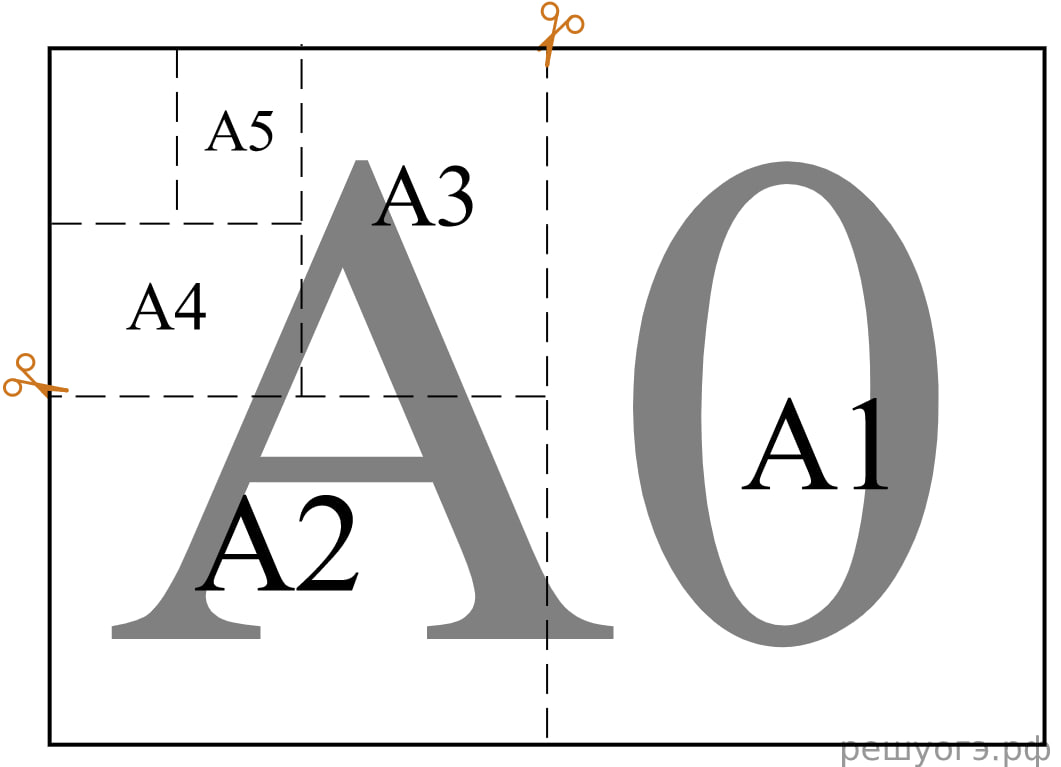
\includegraphics[align=t, width=0.4\linewidth]{../../pics/G91M6L1}
		\end{center}
		Отношение большей стороны к меньшей стороне листа каждого формата одно и то же, поэтому листы всех форматов подобны. Это сделано специально для того, чтобы пропорции текста и его расположение на листе сохранялись при уменьшении или увеличении шрифта при изменении формата листа.
		\item Сколько листов формата \( A3 \) получится из одного листа формата \( A2 \)?
		\item Найдите площадь листа формата \( A1 \). Ответ дайте в квадратных сантиметрах.
		\item Найдите отношение длины меньшей стороны листа формата \( A3 \) к большей. Ответ округлите до десятых.
		\item Бумагу формата \( A5 \) упаковали в пачки по \( 500 \) листов. Найдите массу пачки, если масса бумаги площади \( 1 \) кв. м равна \( 80 \) г. Ответ дайте в граммах.
			\item Решите уравнения:
		\begin{tasks}(2)
			\task \( 2x^2+x=0 \)
			\task \( -3x^2-12x=0 \)
			\task \( 7x^2+14x=0 \)
			\task \( 8x^2+3x=0 \)
			\task \( x^2=64 \)
			\task \( x^2=36 \)
			\task \( -x^2+25=0 \)
			\task \( 100-x^2=0 \)
			\task \( x^2-8x+12=0 \)
			\task \( 15-2x-x^2=0 \)
			\task \( x^2-4x+3=0 \)
			\task \( x^2-4x+4=0 \)
			\task \( 10x^2-17x+34=7x^2-26x+28 \)
			\task \( (x-6)^2=-24x \)
			\task \( x^2+9=(x+9)^2 \)
			\task \( (2x+7)^2=(2x-1)^2 \)
		\end{tasks}
	\end{listofex}
\end{class}
%END_FOLD

%BEGIN_FOLD % ====>>_ Домашняя работа 1 _<<====
\begin{homework}[number=1]
	\begin{listofex}
		\item В таблице даны размеры (с точностью до мм) четырёх листов, имеющих форматы \( A0 \), \( A1 \), \( A3 \), \( A4 \).
		\begin{center}
			\footnotesize
			\begin{tabular}{|c|c|c|}
				\hline
				\rowcolor{gray}\textbf{Номер листа}&\textbf{Длина(мм)}&\textbf{Ширина мм}\\
				\hline
				\( 1 \)&\( 297 \)&\( 210 \)\\
				\hline
				\( 2 \)&\( 420 \)&\( 297 \)\\
				\hline
				\( 3 \)&\( 1189 \)&\( 841 \)\\
				\hline
				\( 4 \)&\( 841 \)&\( 594 \)\\
				\hline
			\end{tabular}
		\end{center}
		Установите соответствие между форматами и номерами листов. В ответ запишите последовательность четырёх цифр, соответствующих номерам листов, без пробелов, запятых и дополнительных символов.
		\begin{center}
			\footnotesize
			\begin{tabular}{|c|c|c|c|}
				\hline
				\textbf{\( A0 \)}&\textbf{\( A1 \)}&\textbf{\( A3 \)}&\textbf{\( A4 \)}\\
				\hline
				\(  \)&\(  \)&\(  \)&\(  \)\\
				\hline
			\end{tabular}
		\end{center}
		Общепринятые форматы листов бумаги обозначают буквой \( A \) и цифрой: \( A0 \), \( A1 \), \( A2 \) и так далее. Лист формата \( A0 \) имеет форму прямоугольника, площадь которого равна \( 1 \) кв. м. Если лист формата А0 разрезать пополам параллельно меньшей стороне, получается два равных листа формата \( A1 \). Если лист \( A1 \) разрезать так же пополам, получается два листа формата \( A2 \). И так далее.
		\begin{center}
			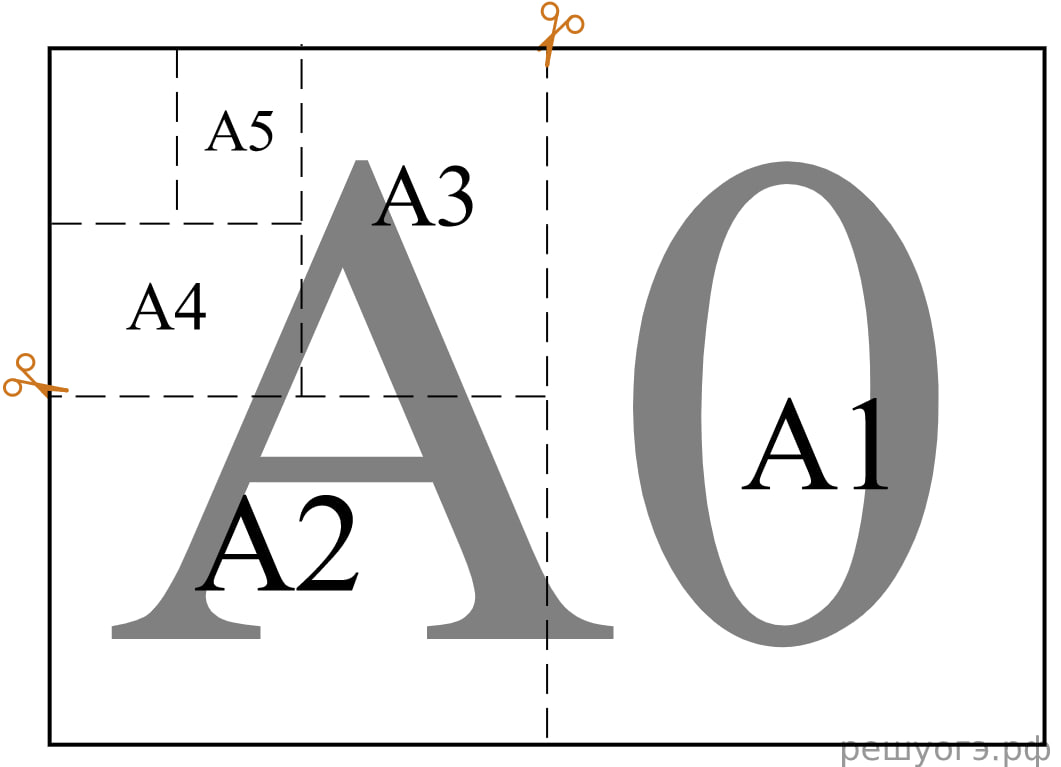
\includegraphics[align=t, width=0.4\linewidth]{../../pics/G91M6L1}
		\end{center}
		Отношение большей стороны к меньшей стороне листа каждого формата одно и то же, поэтому листы всех форматов подобны. Это сделано специально для того, чтобы пропорции текста и его расположение на листе сохранялись при уменьшении или увеличении шрифта при изменении формата листа.
		\item Сколько листов формата \( A5 \) получится из одного листа формата \( A1 \)?
		\item Найдите площадь листа формата \( A6 \). Ответ дайте в квадратных сантиметрах.
		\item Найдите отношение длины большей стороны листа формата \( A2 \) к меньшей. Ответ округлите до десятых.
		\item Бумагу формата \( A3 \) упаковали в пачки по \( 250 \) листов. Найдите массу пачки, если масса бумаги площади \( 1 \) кв. м равна \( 120 \) г. Ответ дайте в граммах.
		\item Решите уравнения:
		\begin{tasks}(2)
			\task \( 2x^2-10x=0 \)
			\task \( x^2+3x=4 \)
			\task \( (x-4)^2+(x+9)^2=2x^2 \)
			\task \( (x+10)^2=(5-x)^2 \)
		\end{tasks}
	\end{listofex}
\end{homework}
%END_FOLD

%BEGIN_FOLD % ====>>_____ Занятие 2 _____<<====
\begin{class}[number=2]
	\begin{listofex}
		\item Найдите все углы, образованные при пересечении параллельных прямых a и b с секущей c, если:
		\begin{tasks}(1)
			\task один из углов равен \(150 \degree\),
			\task один из углов на \(70 \degree\) больше другого.
		\end{tasks}
		\item Докажите, что сумма углов треугольника равна \(180 \degree\).
		\item Через вершину \(B\) треугольника \(ABC\) проведена прямая, параллельная прямой \(AC\). Образовавшиеся при этом три угла с вершиной \(B\) относятся как \(3:10:5\). Найдите углы треугольника \(ABC\).
		\item В параллелограмме \(ABCD\) проведены биссектрисы \(AK\) и \(BN\), которые пересекаются в точке \(Q\). Найти \(\angle AQB\).
		\item В параллелограмме \(ABCD\) углы \(BAC\) и \(CAD\) равны соответственно \(35 \degree\) и \(25 \degree\). Найдите углы \(BAC, ABC, BCA, CDB\).
	\end{listofex}
\end{class}
%END_FOLD

%BEGIN_FOLD % ====>>_ Домашняя работа 2 _<<====
\begin{homework}[number=2]
	\begin{listofex}
		\item Домашняя работа
	\end{listofex}
\end{homework}
%END_FOLD

%BEGIN_FOLD % ====>>_____ Занятие 3 _____<<====
\begin{class}[number=3]
	\begin{listofex}
		\item Занятие 3
	\end{listofex}
\end{class}
%END_FOLD

%BEGIN_FOLD % ====>>_ Домашняя работа 3 _<<====
\begin{homework}[number=3]
	\begin{listofex}
		\item Домашняя работа
	\end{listofex}
\end{homework}
%END_FOLD

%BEGIN_FOLD % ====>>_____ Занятие 4 _____<<====
\begin{class}[number=4]
	\begin{listofex}
		\item Пусто
	\end{listofex}
\end{class}
%END_FOLD


%BEGIN_FOLD % ====>>_ Проверочная работа _<<====
\begin{exam}
	\begin{listofex}
		\item Проверочная
	\end{listofex}
\end{exam}
%END_FOLD